\chapter{HARDNESS TESTING OF METALS}
\section{Experimental targets}
\begin{itemize}
	\item Understand the principle of Brinell, Rockwell and Vicker hardness measurement methods.
	\item Familiar and pracce the common hardness equipment.
\end{itemize}

\section{Theoretical summary}
Hardness tests are performed more frequently than any other mechanical test for several reasons: They are simple and inexpensive-typically, no special specimen need be prepared, and the testing apparatus is relatively inexpensive. The test is non-destructive —the specimen is neither fractured nor excessively deformed;  a  small  indentation  is  the  only  deformation.  Other  mechanical  properties  often  may  be estimated from hardness data, such as tensile strength.
\subsection{Brinell Hardness Test}
A hard, spherical indenter is forced into the surface of the metal to be tested. The diameter of the hardened steel (or tungsten carbide) indenter is 10.00 mm (0.394 in.). Standard loads range between 500 and 3000 kg in 500-kg increments; during a test, the load is maintained constant for a specified me (between 10 and 30 s). Harder materials require greater applied loads. The Brinell hardness number, HB, is a function of both the magnitude of the load and the diameter of the resulting indentation . This diameter  is  measured  with  a  special  low-power  microscope,  utilizing  a  scale  that  is  etched  on  the eyepiece. The measured diameter is then converted to the appropriate HB number using a chart; only one scale is employed with this technique.
\subsection{Rockwell Hardness Tests}
Indenters include spherical and hardened steel balls having diameters of 1/16, 1/8, ¼, and 12 in. (1.588, 3.175, 6.350, and 12.70 mm, respectively), as well as a conical diamond (Brale) indenter, which is used for the hardest materials. With this system, a hardness number is determined by the difference in depth of penetration resulting from the application of an initial minor load followed by a larger major load; utilization of a minor load enhances test accuracy. On the basis of the magnitude of both major and minor loads, there are two types of tests: Rockwell and superficial Rockwell. For the Rockwell test, the minor  load is  10  kg, whereas major  loads are 60, 100, and 150 kg. When specifying  Rockwell  and superficial  hardnesses,  both  hardness  number  and  scale  symbol  must  be  indicated.  The  scale  is designated by the symbol HR followed by the appropriate scale identification.
\subsection{Knoop and Vickers Microindentation Hardness Tests}
Use a very small diamond indenter having pyramidal geometry is forced into the surface of the specimen. Applied loads are much smaller than for the Rockwell and Brinell tests, ranging between 1 and 1000 g. The resulting impression is observed under a microscope and measured; this measurement is then converted into a hardness number. The Knoop and Vickers hardness numbers are designated by HK and HV, respectively, and hardness scales for both techniques are approximately equivalent. Both are well suited for measuring the hardness of small, selected specimen regions; furthermore, the Knoop technique is used for testing brittle materials such as ceramics.
\subsection{Hardness Conversion}
Have been determined experimentally and found to be dependent on material type and characteristics. The most reliable conversion data exist for steels, some of which are presented in Figure 1.4 for Knoop, Brinell, and two Rockwell scales; the Mohs scale is also included. Detailed conversion tables for various other metals and alloys are contained in ASTM Standard E140, “Standard Hardness Conversion Tables for  Metals”.  In  light  of  the  preceding  discussion,  care  should  be  exercised  in  the  extrapolation  of conversion data from one alloy system to another.

\section{Detailed Experiment}
\subsection{Measure HR}
Put sample on the flat form of the equipment (anvil). Setting force application, Rockwell indentor conditions (HRA, HRB, HRC). Rotate clockwise the control to lift the flat form of the equipment until the sample touches the indentor. Continue rotating the control until the short hand rotates the red position. Rotating the watch face so that the long hand points at C-B position . Press start button, waiting in 10s (duration of applying force). After 10s, a “beep” sound is released. The position of the long hand shows the measured value. Notice that, the black outside cycle is HRA, HRC and the red inside cycle indicates HRB. Rounding values to 0.5. - Rotate counterclockwise the control to release the sample and repeat the measurement for other 2 mes (3 measured points are close to avoid the error due to uneven hardness.
\subsection{Measure HB or HV}
Put sample on the flat form of the equipment. Rotate clockwise the control to li the flat form of the equipment until the sample touches the indentor. Continue rotating the control until the needle moves to the end of the ruler. Lower gently the force control bar to the end of the range and wait for 10 seconds then lifting up the force control bar lightly. - Rotate clockwise the control to release the sample. Mark on the measured dimple by the pen. This process was repeated other 2 mes. - Take one of the three holes to measure diagonal length D (for HV method) or the concave diameter D (for HB method) by using optical measurement. The other two holes will be measured on the microscope and the data will be upload on the web page of the Material Processing Department. Then, students download data and complete the report.
\begin{figure}
	\centering
	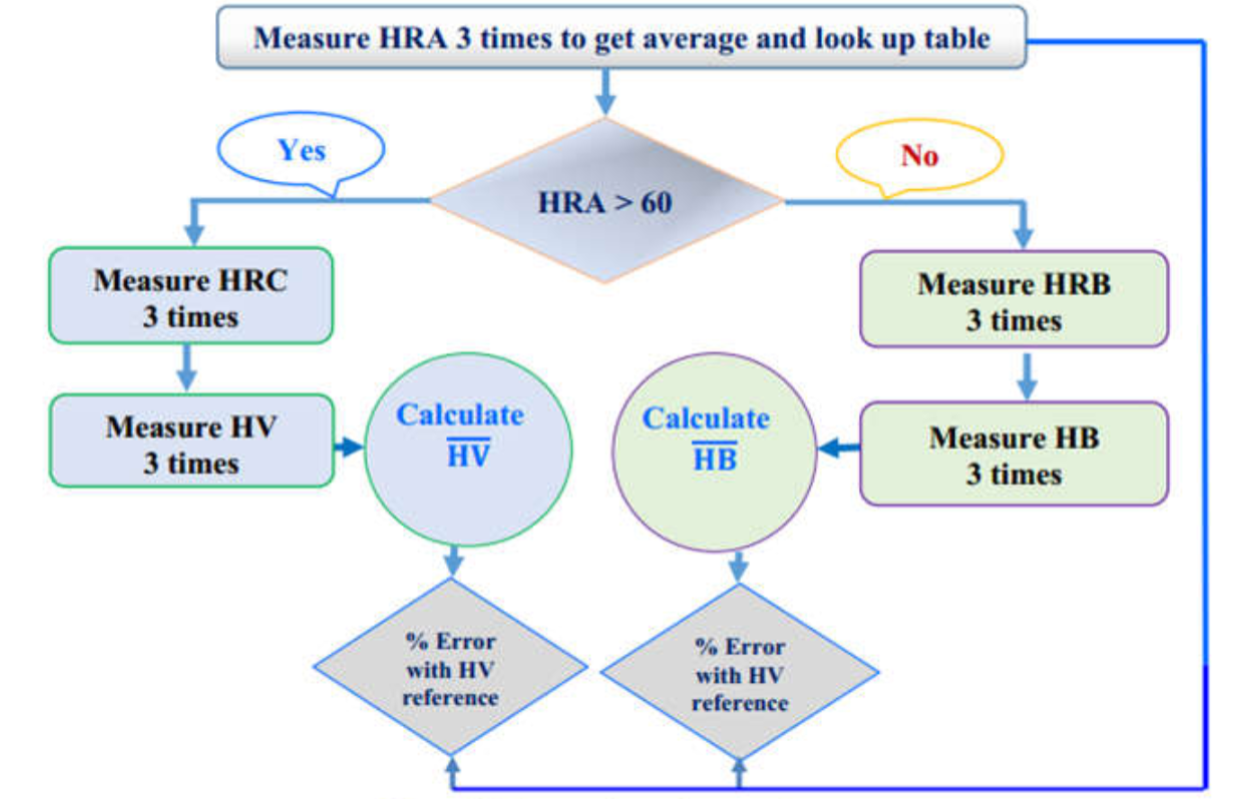
\includegraphics[width=150mm]{2020-07-19 14.04.25 oemmndcbldboiebfnladdacbdfmadadm 4d3397925039.png}
	\caption{Measured practice procedure}
\end{figure}\clearpage

\section{Measurement results}
\begin{figure}[ht]
	\centering
	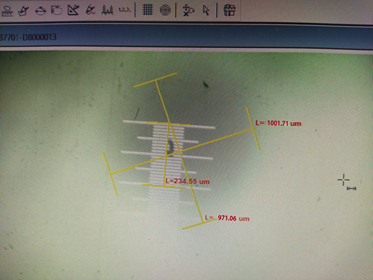
\includegraphics[width=150mm]{109267072_710156266492754_8636426261719016576_n.png}
	\caption{Experimental results of the diagonal lines}
	\label{1}
\end{figure}
\begin{table}[ht]
	\centering
	\renewcommand{\arraystretch}{1.5}
	\begin{tabular}{llrrrr}
		\toprule
		\multicolumn{2}{c}{Properties}                   &$ 1^{st} $ measure  & \multicolumn{1}{c}{$ 2^{nd} $ measure} & \multicolumn{1}{c}{$ 3^{rd} $ measure} & \multicolumn{1}{c}{Avg} \\ \midrule
		\rowcolor{lightgray!20}\multicolumn{2}{l}{\cellcolor[HTML]{C0C0C0}HRA }&- {\color[HTML]{C0C0C0} } &-  & - &- \\ 
		\multicolumn{2}{l}{\cellcolor[HTML]{C0C0C0}HRB/HRC} &106/27   & 106/30 & 103/27 & 105/28 \\ 
		\rowcolor{lightgray!20}\cellcolor[HTML]{C0C0C0} & Diagonal line \cellcolor[HTML]{EFEFEF} & HOLE 1 & HOLE 2 & HOLE 3 & - \\  
		\cellcolor[HTML]{C0C0C0} & \cellcolor[HTML]{EFEFEF} $ D_1 $ & 0.846 & 0.833& 0.815 & -\\  
		\rowcolor{lightgray!20}{\cellcolor[HTML]{C0C0C0} } & \cellcolor[HTML]{EFEFEF} $ D_2 $ & 0.872 & 0.859 & 0.841 & -\\  
		\multirow{-4}{*}{\cellcolor[HTML]{C0C0C0}HV/HB } & \cellcolor[HTML]{EFEFEF}Avg  &   0.859                      &          0.846               &    0.828        & -             \\ \hline
	\end{tabular}
	\caption{Measurement results}
	\label{3}
\end{table}

\section{Analyzing results}

\paragraph{Lookup table} We look up the table according to the website:\\ \textit{https://www.steelexpress.co.uk/steel-hardness-conversion.html}
\begin{figure}[ht]
	\centering
	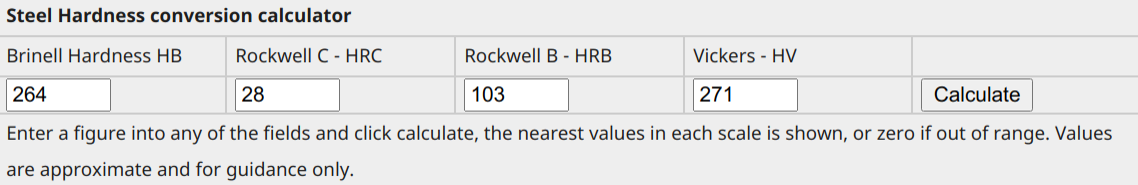
\includegraphics[width=150mm]{2020-07-19 14.08.38 oemmndcbldboiebfnladdacbdfmadadm cba70144e432.png}
	\caption{Lookup table}
	\label{2}
\end{figure}\\
$ \Rightarrow HV_{theory} = 271 $
\paragraph{Calculate average HV} The results are as follows (Let $ P=980\unit{(N)} $):\\
$ HV_1 = \dfrac{2P\sin\left(\dfrac{136^\circ}{2}\right)}{9.81\overline{D}_1^2} = 251.1 $\\
$ HV_2 = \dfrac{2P\sin\left(\dfrac{136^\circ}{2}\right)}{9.81\overline{D}_2^22} = 258.8 $\\
$ HV_3 = \dfrac{2P\sin\left(\dfrac{136^\circ}{2}\right)}{9.81\overline{D}_3^2} = 270.2 $\\
$ \overline{HV} = \dfrac{HV_1+HV_2+HV_3}{3} = 260 $\\
$ \delta = \dfrac{|HV_{theory}-\overline{HV}|}{HV_{theory}}\times100\% = 4.06\% $

\section{Conclusion}
Based on experimental data, the error between reality and theory when measuring the HRC hardness of the sample is very small, only about $ 4.06\% $ and when measuring HV hardness, the error between reality and theory is also very small ( $ 4.06\% $) and negligible
\paragraph{Explanaon about errors} $ $
\begin{itemize}
	\item Due to laboratory equipment, machines and instruments, the integrity of the prick, the load of the machine, the inclination of the work piece surface, the error of the indicator.
	\item Due to the measurer's estimation of the indicator data on the meter.
	\item Due to rounding.
	\item Because the surface of the sample has not been carefully grounded.
	\item Because the placement of the prick is not reasonable.
	\item Due to the uneven holding me between measurements.
	\item Due to the meter calibration is not good.
	\item Due to the inaccurate determination of line d, it causes errors in HV hardness.
	\item Due to the lifting of the booms, the rhythm of the measuring hole is not smooth.
\end{itemize}